\section{Exploiting the Dynamic Structure for Latent Space Control}\label{sec:con:latent_space_control}

We consider the problem setting of guiding the system towards a desired observation $o^\mathrm{d}$ by providing a sequence of inputs $u(t_k)$ such that at time $t_N$, the actual observation $o(t_N)$ matches $o^\mathrm{d}$.
% Performing control in latent space drastically reduces the algorithmic requirements as $n_z \ll h_\mathrm{o} \, w_\mathrm{o}$.
A relatively simple way would be to encode the desired observation into latent space $z^\mathrm{d} = \Phi(o^\mathrm{d})$ and then to design a feedback controller (e.g., PID) in latent space: $g(u) = \mathrm{PID}(z^\mathrm{d}-z(t), -\dot{z})$.
Unfortunately, several challenges appear: first, it is not clear how the latent-space force $\tau = g(u)$ can be mapped back to an actual input $u(t)$ as the inverse input-to-forcing mapping $g^{-1}$ is generally not known.
Furthermore, relying entirely on a PID controller has several well-known drawbacks, such as poor and slow transient behavior, steady-state errors (in case the integral gain is chosen to be zero), and instability for high proportional and integral gains.
% Another option would be to formulate a \gls{MPC} optimization problem~\cite{lenz2015deepmpc, hafner2019learning, hewing2020learning, alora2023robust} and find the optimal input sequence on the chosen horizon to guide the system towards $o^\mathrm{d}$. This has disadvantages, too, as the computational requirements are considerable, and it can be difficult to tune cost functions in latent space.
% In this work, we propose a control strategy that can solve or sidestep all the challenges mentioned above.
We take inspiration from potential shaping strategies~\cite{bloch2001controlled, ortega2021pid}, which are widely used for effectively controlling (elastic) robots, and, therefore, combine a feedforward term compensating the latent-space potential forces with an integral-saturated, PID-like feedback term. For mapping the desired forcing $\tau$ back to an input $u(t)$, we train an forcing decoder $\eta: \mathbb{R}^{n} \to \mathbb{R}^{m}$ that approximates $g^{-1}$. Specifically, we consider here the structure $u = \eta(\tau) = E(\tau) \, \tau$, where $E \in \mathbb{R}^{m \times n}$ is parameterized by an \gls{MLP}.

\subsection{Control strategy}
The latent-space control law is given by
\begin{equation}\label{eq:con:controller}
    \tau(t) = g(u) = \underbrace{K_\mathrm{w} \, z^\mathrm{d} + \tanh(z^\mathrm{d} + b)}_{\substack{\text{Feedforward term:}\\ \text{compensation of potential forces}}} + \underbrace{K_\mathrm{p} \, (z^\mathrm{d} - z) - K_\mathrm{d} \, \dot{z} + K_\mathrm{i} \int_0^t \tanh(\upsilon (z^\mathrm{d}(t') - z(t')))\mathrm{d}t'}_{\text{Feedback term: P-satI-D}}
\end{equation}
where $K_\mathrm{p}, K_\mathrm{i}, K_\mathrm{d} \in \mathbb{R}^{n \times n}$ are the proportional, integral, and derivative control gains, respectively.
As integral terms can often lead to instability when applied to nonlinear systems~\cite{stolzle2024experimental}, we adopt an integral term saturation~\cite{pustina2022p} with the associated dimensionless gain $\upsilon \in \mathbb{R}$, which ensures that the integral error added at each time step is bounded to the interval $(-1, 1)$.
% 
Subsequently, $\tau$ is  decoded to the input as $u(t) = \eta(\tau) = E(\tau) \, \tau$.
For training this decoder, we add a reconstruction loss to \eqref{eq:training_loss}: $\mathcal{L}_{\mathrm{u}}(t_k) = \lambda_{\mathrm{u}} \, \mathrm{MSE}(u(t_k), \hat{u}(t_k)) = \lambda_{\mathrm{u}} \, \mathrm{MSE} \left (u(t_k), \eta(g(u(t_k))) \right )$.

\begin{figure}[t]
    \centering
    \subfigure[Samples of used datasets]{\includegraphics[width=0.27\linewidth]{con/figures/datasets_visualization/datatsets_visualization_v2_cropped_compressed.pdf}\label{fig:con:datasets_visualization}}
    \hfill
    \subfigure[Blockscheme of model-based control in latent space]{\includegraphics[width=0.69\linewidth]{con/figures/control/blockdiagram_latent_space_control_v1_cropped.pdf}\label{fig:con:blockdiagram_latent_space_control}}
    \caption{\textbf{Panel (a):} Samples of some of the datasets used as part of the experimental verification, specifically for the results reported in Tab.~\ref{tab:con:latent_dynamics_results}. The real-world Reaction-Diffusion image is adopted from~\cite{epstein2016reaction}. \textbf{Panel (b):} Model-based control in latent space by exploiting the physical structure of the CON model.}
\end{figure}

\subsection{Implementation of closed-loop control}
We generate a trajectory of $7$ setpoints, where $q^\mathrm{d}(t_j) \in \mathbb{R}^{n_\mathrm{q}}$ is a sampled configuration of the actual system.
Then, we render an image $o^\mathrm{d}(t_j)$ that represents the target observation for the controller and encode it into latent space to retrieve $z^\mathrm{d} \in \mathbb{R}^{n_\mathrm{z}}$.
At time step $k$, we render an image $o(t_k)$ of the robot's current configuration $q(t_k)$ and encode the image. 
% Analog to Section~\ref{sec:con:learning_latent_space_dynamics}, we apply finite differences in image space to retrieve an estimate of $\hat{\dot{o}}$ and then project into latent space to capture the latent velocity $\dot{z}$. % that is needed by the control law in case the derivative feedback terms are active.
Subsequently, we evaluate the control law and apply the decoder $u(t_k) = \eta(\tau(t_k)))$, which is finally passed to the simulator that integrates the ground-truth dynamics to the next time-step $t_{k+1}$ considering the actuation $u(t_k)$.
The controller runs at \SI{100}{Hz}, and we simulate the ground-truth dynamics with a \emph{Dopri5} \gls{ODE} integrator at a time-step of \num{5e-4}~\si{s}.

\subsection{Latent-space control of a damped harmonic oscillator}

We consider an actuated version of the \emph{M-SP+F} dataset (i.e., a damped harmonic oscillator) and denote it with \emph{M-SP+F+A}. All system, trajectory sampling and rendering parameters remain the same, except that for each trajectory in the dataset we randomly sample a forcing $u \sim \mathcal{U}(-\SI{1}{N}, \SI{1}{N})$.

We train a \gls{CON} model with latent dimension $n_z = 1$ over three random seeds on the \emph{M-SP+F+A} dataset. This means that the network consists of a single oscillator.
From the three different random seeds, we choose the model that achieves the best validation loss, which results in an RMSE of $0.0327$, a PSNR of $5.99$, and SSIM of $0.9796$ on the test set.

Fig.~\ref{fig:con:control:m-sp+f+a:analysis} shows how the encoder learns an almost linear relationship between the actual configuration of the system and the predicted latent space representation. Furthermore, we notice that both the ground-truth and the learned potential energy are convex and exhibit a global minimum at $q=\SI{0}{m}$.

We compare the performance of \emph{P-satI-D}, \emph{D+FF}, and \emph{P-satI-D+FF} controllers based on the \gls{CON} model in Fig.~\ref{fig:con:control:m-sp+f+a:sequences_comparison}.
For the \emph{P-satI-D} controller, we choose the control gains $K_\mathrm{p} = 10, K_\mathrm{i}=10, K_\mathrm{d} = \num{5}, \upsilon = 1$. The \emph{D+FF} controller uses $K_\mathrm{d} = \num{3.5}$. Finally, the \emph{P-satI-D+FF} is configured with $K_\mathrm{p} = 2, K_\mathrm{i}=0.3, K_\mathrm{d} = \num{3.5}, \upsilon = 1$.
The results show that the \emph{P-satI-D+FF} controller exhibits thanks to its feedforward term no overshooting and a faster response time than the pure feedback controller \emph{P-satI-D}. The high accuracy of the feedfoward term can be seen from the performance of the \emph{D+FF} controller, that only exhibits relatively small steady-state error. Adding small proportional and integral feedback actions in the \emph{P-satI-D+FF} controller keeps the compliance high while removing the steady-state error and reducing the response time.

Finally, we visualize the behavior of the \emph{P-satI-D+FF} controller as a sequence of stills in Fig.~\ref{fig:con:control:m-sp+f+a:con_PsatID+FF:sequence_of_stills}.


\begin{figure}[ht]
    \centering
    \subfigure[Configuration $q$ to latent $z$ mapping]{\includegraphics[width=0.49\columnwidth, trim={5, 10, 5, 5}]{con/figures/results/control/m-sp+f+a/analysis/mapping_configuration_to_latent_space.pdf}}
    \subfigure[Ground-truth and learned potential energy $\mathcal{U}$]{\includegraphics[width=0.49\columnwidth, trim={5, 10, 5, 5}]{con/figures/results/control/m-sp+f+a/analysis/potential_energy_landscape_q.pdf}}
    \caption{
    \textbf{Panel (a):} Learned mapping from configuration to latent space for the CON model with $n_z$ (i.e., consisting of a single oscillator) trained on the actuated damped harmonic oscillator (\emph{M-SP+F+A}) dataset. \textbf{Panel (b):} The blue line represents the ground-truth potential energy of the damped harmonic oscillator. The orange line represents the learned potential energy of the CON model evaluated vs. the system configuration by rendering and subsequently encoding into latent space each configuration value.
    }\label{fig:con:control:m-sp+f+a:analysis}
\end{figure}

\begin{figure}[ht]
    \centering
    \subfigure[Configuration $q(t) \in \mathbb{R}^2$]{\includegraphics[width=0.49\columnwidth, trim={5, 10, 5, 5}]{con/figures/results/control/m-sp+f+a/analysis/setpoint_control_sequences_q.pdf}}
    \subfigure[Latent representation $z(t) \in \mathbb{R}^2$]{\includegraphics[width=0.49\columnwidth, trim={5, 10, 5, 5}]{con/figures/results/control/m-sp+f+a/analysis/setpoint_control_sequences_z.pdf}}\\
    \subfigure[Control input $u(t) \in \mathbb{R}^2$]{\includegraphics[width=0.49\columnwidth, trim={5, 10, 5, 5}]{con/figures/results/control/m-sp+f+a/analysis/setpoint_control_sequences_u.pdf}}
    \subfigure[Potential energy $U(t) \in \mathbb{R}$]{\includegraphics[width=0.49\columnwidth, trim={5, 10, 5, 5}]{con/figures/results/control/m-sp+f+a/analysis/setpoint_control_sequences_potential_energy.pdf}}
    \caption{Latent-space control of an actuated damped harmonic oscillator (\emph{M-SP+F+A}) following a sequence of setpoints. 
    We compare multiple controllers based on a trained \gls{CON} network with $n_z=1$. The \gls{CON} model weights are initialized using a random seed of 0.
    The blue line represents a pure feedback controller (\emph{P-satI-D}). The orange line visualizes the behavior of a feedforward controller with only a damping term applied in feedback (\emph{D+FF}). The green line shows the performance of our proposed combination of feedback and feedforward terms (\emph{P-satI-D+FF}).
    The dotted and solid lines show the reference and actual values, respectively.
    For each setpoint, we randomly sample a desired shape $q^\mathrm{d}$ and render the corresponding image $o^\mathrm{d}$. This image is then encoded to a target latent $z^\mathrm{d}$. The controller then computes a latent-space torque $F^\mathrm{d}$, which is decoded to an input $u$. Finally, we provide this input to the simulator, which performs a roll-out of the closed-loop dynamics.
    Important: The robot's configuration (i.e., the first-principle, minimal-order state) is solely used for generating a target image and simulating the closed-loop system. 
    }\label{fig:con:control:m-sp+f+a:sequences_comparison}
\end{figure}

\begin{figure}[hb]
    \centering
    \subfigure[t=\SI{0.0}{s}]{\includegraphics[width=0.16\columnwidth]{con/figures/results/control/m-sp+f+a/con_psatid+ff/sequences_of_stills/setpoint_sequence_controlled_rollout_actual_0.00.png}}
    \subfigure[t=\SI{0.5}{s}]{\includegraphics[width=0.16\columnwidth]{con/figures/results/control/m-sp+f+a/con_psatid+ff/sequences_of_stills/setpoint_sequence_controlled_rollout_actual_0.50.png}}
    \subfigure[t=\SI{1.0}{s}]{\includegraphics[width=0.16\columnwidth]{con/figures/results/control/m-sp+f+a/con_psatid+ff/sequences_of_stills/setpoint_sequence_controlled_rollout_actual_1.00.png}}
    \subfigure[t=\SI{1.5}{s}]{\includegraphics[width=0.16\columnwidth]{con/figures/results/control/m-sp+f+a/con_psatid+ff/sequences_of_stills/setpoint_sequence_controlled_rollout_actual_1.50.png}}
    \subfigure[t=\SI{2.0}{s}]{\includegraphics[width=0.16\columnwidth]{con/figures/results/control/m-sp+f+a/con_psatid+ff/sequences_of_stills/setpoint_sequence_controlled_rollout_actual_2.00.png}}
    \subfigure[Target $0-4.9\si{s}$]{\includegraphics[width=0.16\columnwidth]{con/figures/results/control/m-sp+f+a/con_psatid+ff/sequences_of_stills/setpoint_sequence_controlled_rollout_desired_0.00.png}}
    \\
    \subfigure[t=\SI{5.00}{s}]{\includegraphics[width=0.16\columnwidth]{con/figures/results/control/m-sp+f+a/con_psatid+ff/sequences_of_stills/setpoint_sequence_controlled_rollout_actual_5.00.png}}
    \subfigure[t=\SI{5.5}{s}]{\includegraphics[width=0.16\columnwidth]{con/figures/results/control/m-sp+f+a/con_psatid+ff/sequences_of_stills/setpoint_sequence_controlled_rollout_actual_5.50.png}}
    \subfigure[t=\SI{6.0}{s}]{\includegraphics[width=0.16\columnwidth]{con/figures/results/control/m-sp+f+a/con_psatid+ff/sequences_of_stills/setpoint_sequence_controlled_rollout_actual_6.00.png}}
    \subfigure[t=\SI{6.5}{s}]{\includegraphics[width=0.16\columnwidth]{con/figures/results/control/m-sp+f+a/con_psatid+ff/sequences_of_stills/setpoint_sequence_controlled_rollout_actual_6.50.png}}
    \subfigure[t=\SI{7.5}{s}]{\includegraphics[width=0.16\columnwidth]{con/figures/results/control/m-sp+f+a/con_psatid+ff/sequences_of_stills/setpoint_sequence_controlled_rollout_actual_7.00.png}}
    \subfigure[Target $5-9.9\si{s}$]{\includegraphics[width=0.16\columnwidth]{con/figures/results/control/m-sp+f+a/con_psatid+ff/sequences_of_stills/setpoint_sequence_controlled_rollout_desired_5.00.png}}
    \caption{Sequence of closed-loop control of an actuated damped harmonic oscillator (\emph{M-SP+F+A}) with a \emph{P-satI-D+FF}controller  based on a trained \gls{CON} with $n_z=1$.
    \textbf{Columns 1-4:} show the actual behavior of the closed-loop system. \textbf{Column 5:} demonstrates the target image that the control sees for all time instances in the row.
    }\label{fig:con:control:m-sp+f+a:con_PsatID+FF:sequence_of_stills}
\end{figure}

\subsection{Latent-space control of a two segment PCC soft robot}

\subsubsection{Experimental setup.}
% After initializing the neural network weights with three different random seeds, 
We train a \gls{CON} model with two latent variables ($n_z = 2$) on the \emph{PCC-NS-2} dataset.
Analog to the input encoder mapping $B(u)$, the forcing decoder mapping $E(\tau)$ is parametrized by an \gls{MLP} consisting of five layers with hidden dimension $30$ and a hyperbolic tangent activation function.
The \emph{CON} model achieves an \gls{RMSE} of $0.1628$ on the test set.
\subsubsection{Model selection}
For the control experiments, we train instances of the \emph{MECH-NODE} and \emph{CON-M} models with latent dimension $n_z = 2$ and with neural network weights initialized with three different random seeds. 
We found that model-based control does not perform as well when the latent stiffness $\Gamma_\mathrm{w}$ (as visualized in Fig.~\ref{fig:con:control:pcc_ns-2:potential_energy_landscape_z}) is significantly larger along one of the Eigenvectors than along the other one. Therefore, we evaluate the Eigenvalues of the learned stiffness matrix in $\mathcal{W}$-coordinates after training: $\lambda_{1,2}(\Gamma_\mathrm{w})$. Particularly, we choose the seed that minimizes the normalized standard deviation of the Eigenvalues: $\mathrm{seed} = \arg\min \frac{\sigma_\lambda}{\mu_\lambda}$, where
\begin{equation}
\begin{split}
    \mu_\lambda = \frac{\lambda_1(\Gamma_\mathrm{w}) + \lambda_2(\Gamma_\mathrm{w})}{2},
    \quad
    \sigma_\lambda = \sqrt{\frac{(\lambda_1(\Gamma_\mathrm{w})-\mu_\lambda)^2 + (\lambda_2(\Gamma_\mathrm{w})-\mu_\lambda)^2}{2}}.
\end{split}
\end{equation}


We benchmark two controllers on the simulated continuum soft robot consisting of two segments: (i) a pure \emph{P-satI-D} controller (i.e., the feedback term in \eqref{eq:con:controller}) that leverages the smooth mapping into the latent representation enabled by the \gls{CON} dynamic model and the $\beta$-\gls{VAE}, and (ii) a \emph{P-satI-D+FF} (i.e., \eqref{eq:con:controller}) that exploits the structure of the \gls{CON} dynamics by compensating for the potential forces.
The stable closed-loop system dynamics made the control gain tuning very easy, and we selected $K_\mathrm{p} = 1, K_\mathrm{i}=2, K_\mathrm{d} = 0.02, \upsilon = 1$ for the \emph{P-satI-D} controller and $K_\mathrm{p} = 0, K_\mathrm{i}=2, K_\mathrm{d} = 0.05, \upsilon = 1$ for the \emph{P-satI-D+FF} controller, respectively.

Furthermore, we compare the control performance of our model-based controllers with a baseline control strategy based on the \emph{MECH-NODE} ($n_z = 2$) that achieves an error of $0.1104$ on the test set.
For \emph{MECH-NODE}, we chose the model with the lowest validation loss (seed $0$)
First, we utilize the same P-satI-D feedback controller as for the \gls{CON} model to generate the control action $\tau(t)$ in latent space. 
As the MECH-NODE uses an \gls{MLP} to parameterize the function $\dot{\xi} = f_\xi(\xi, u)$, we cannot easily map $\tau(t)$ into an input $u(t)$. 
Therefore, we linearize the latent space dynamics w.r.t to the input as $f_{\xi,\mathrm{ac}}(\xi, u) = f_\xi(\xi, 0) + A(\xi) \, u$, where $A(\xi) = \frac{\partial f_\xi}{\partial u}(\xi, 0)$ is computed using autodiff. Then, $u(t) = A^\mathrm{T}(\xi) \, \tau(t)$. After tuning the control gains, we choose  $K_\mathrm{p} = 0.001, K_\mathrm{i}=0.02, K_\mathrm{d} = \num{1e-5}, \upsilon = 1$.
% Therefore, we leverage auto differentiation to linearize the system dynamics w.r.t. the input $u$

\subsubsection{Potential energy landscape}
When leveraging (learned) dynamical models for setpoint regulation, it is essential to accurately estimate the potential energy as this dictates the efficacy of the feedforward terms. Therefore, we qualitatively evaluate the potential energy landscape of the \gls{CON} latent dynamic model.

In Fig.~\ref{fig:con:control:pcc_ns-2:potential_energy_landscape_z}, we can see how \gls{CON} contains a single, isolated, and globally asymptotically stable equilibrium as proven in Section~\ref{sec:con:con}, respectively. 
% 
Furthermore, we want to verify that the learned potential corresponds to the actual potential energy of the simulated system.
An autonomous continuum soft robot with the tip pointing downwards in a straight configuration exhibits an isolated, globally asymptotically stable equilibrium at $q = 0$ (i.e., zero strains)~\cite{stolzle2021piston}.
For this purpose, we can compare the learned potential energy field in Fig.~\ref{fig:con:control:pcc_ns-2:potential_energy_landscape_q} with the ground-truth potential energy field in Fig.~\ref{fig:con:control:pcc_ns-2:potential_energy_landscape_q_gt}.
We confirm, based on Fig.~\ref{fig:con:control:pcc_ns-2:potential_energy_landscape_q}, that, indeed, the learned potential also has its minimum close to/at $q=0$. Although the field is shaped slightly differently, the potential forces are clearly pointing inwards towards the global attractor.

\begin{figure}[ht]
    \centering
    \subfigure[Learned potential energy as a function of $z$]{\includegraphics[width=0.5\columnwidth, trim={5, 10, 5, 5}]{con/figures/results/control/pcc_ns-2/potential_energy_landscape/potential_energy_landscape_z.pdf}\label{fig:con:control:pcc_ns-2:potential_energy_landscape_z}}\\
    \subfigure[Learned potential energy as a function of $q$]{\includegraphics[width=0.49\columnwidth, trim={20, 10, 20, 20}]{con/figures/results/control/pcc_ns-2/potential_energy_landscape/potential_energy_landscape_q.pdf}\label{fig:con:control:pcc_ns-2:potential_energy_landscape_q}}
    \subfigure[Ground-truth potential energy as a function of $q$]{\includegraphics[width=0.49\columnwidth, trim={20, 10, 20, 20}]{con/figures/results/control/pcc_ns-2/potential_energy_landscape/potential_energy_landscape_q_gt.pdf}\label{fig:con:control:pcc_ns-2:potential_energy_landscape_q_gt}}
    \caption{Potential energy landscapes of a \gls{CON} with $n_z=2$ trained to learn the latent space dynamics of a continuum soft robots (simulated with two \gls{PCC} segments). \textbf{Panel (a):} Here, we visualize the learned potential energy of \gls{CON} using the color scale as a function of the latent representation $z = x_\mathrm{w} \in \mathbb{R}^2$. The arrows denote the gradient of the potential field $\frac{\partial \mathcal{U}}{\partial z}$ (i.e., the potential force), with the magnitude of the gradient expressed as the length of the arrow. \textbf{Panel (b):} Again, we display the learned potential energy of \gls{CON} using the color scale, but in this case, as a function of the configuration $q \in \mathbb{R}$ of the robot (that is hidden from the model). First, we render an image $o$ of the shape of the robot for each configuration $q = \begin{bmatrix}
        q_1 & q_2
    \end{bmatrix}^\mathrm{T} \in \mathbb{R}^2$. Then, we encode the image into latent space as $z = \Phi(o)$. This allows us then to compute the potential energy $\mathcal{U}(z)$ of the \gls{CON} latent dynamics model. \textbf{Panel (c):} Here, we display the potential energy and its associated potential forces of the actual (i.e., simulated) system.}
\end{figure}

\begin{figure}[ht]
    \centering
    \subfigure[Config. for P-satI-D with MECH-NODE.]{\includegraphics[width=0.45\columnwidth, trim={5, 10, 5, 5}]{con/figures/results/control/pcc_ns-2/mech_node_psatid/setpoint_control_sequence_q.pdf}}
    \subfigure[Latent for P-satI-D with MECH-NODE.]{\includegraphics[width=0.45\columnwidth, trim={5, 10, 5, 5}]{con/figures/results/control/pcc_ns-2/mech_node_psatid/setpoint_control_sequence_z.pdf}}\\
    \subfigure[Configuration for P-satI-D with \gls{CON}.]{\includegraphics[width=0.45\columnwidth, trim={5, 10, 5, 5}]{con/figures/results/control/pcc_ns-2/con_psatid/setpoint_control_sequence_q.pdf}}
    \subfigure[Latent for P-satI-D with \gls{CON}.]{\includegraphics[width=0.45\columnwidth, trim={5, 10, 5, 5}]{con/figures/results/control/pcc_ns-2/con_psatid/setpoint_control_sequence_z.pdf}}\\
    \subfigure[Configuration for P-satI-D+FF with \gls{CON}.]{\includegraphics[width=0.45\columnwidth, trim={5, 10, 5, 5}]{con/figures/results/control/pcc_ns-2/con_psatid+ff/setpoint_control_sequence_q.pdf}}
    \subfigure[Latent for P-satI-D+FF with \gls{CON}.]{\includegraphics[width=0.45\columnwidth, trim={5, 10, 5, 5}]{con/figures/results/control/pcc_ns-2/con_psatid+ff/setpoint_control_sequence_z.pdf}}\\
    \caption{Latent-space control of a continuum soft robot (simulated using two piecewise constant curvature segments) at following a sequence of setpoints: The upper two rows show the performance of a pure P-satI-D feedback controller operating in latent space $z$ learned with the MECH-NODE and \gls{CON} models, respectively. The lower row displays the results for a latent space controller based on the \gls{CON} model that additionally also compensates for the learned potential forces.}\label{fig:con:latent_space_control_results}
\end{figure}

\begin{figure}[hb]
    \centering
    % image size: 575x575px
    \subfigure[t=\SI{0.0}{s}]{\includegraphics[width=0.16\columnwidth]{con/figures/results/control/pcc_ns-2/con_psatid+ff/sequences_of_stills/setpoint_sequence_controlled_rollout_actual_0.00.png}}
    \subfigure[t=\SI{0.2}{s}]{\includegraphics[width=0.16\columnwidth]{con/figures/results/control/pcc_ns-2/con_psatid+ff/sequences_of_stills/setpoint_sequence_controlled_rollout_actual_0.20.png}}
    \subfigure[t=\SI{0.4}{s}]{\includegraphics[width=0.16\columnwidth]{con/figures/results/control/pcc_ns-2/con_psatid+ff/sequences_of_stills/setpoint_sequence_controlled_rollout_actual_0.40.png}}
    \subfigure[t=\SI{0.6}{s}]{\includegraphics[width=0.16\columnwidth]{con/figures/results/control/pcc_ns-2/con_psatid+ff/sequences_of_stills/setpoint_sequence_controlled_rollout_actual_0.60.png}}
    \subfigure[t=\SI{0.8}{s}]{\includegraphics[width=0.16\columnwidth]{con/figures/results/control/pcc_ns-2/con_psatid+ff/sequences_of_stills/setpoint_sequence_controlled_rollout_actual_0.80.png}}
    \subfigure[Target $0-4.9\si{s}$]{\includegraphics[width=0.16\columnwidth]{con/figures/results/control/pcc_ns-2/con_psatid+ff/sequences_of_stills/setpoint_sequence_controlled_rollout_desired_0.00.png}}
    \\
    \subfigure[t=\SI{5.00}{s}]{\includegraphics[width=0.16\columnwidth]{con/figures/results/control/pcc_ns-2/con_psatid+ff/sequences_of_stills/setpoint_sequence_controlled_rollout_actual_5.00.png}}
    \subfigure[t=\SI{5.2}{s}]{\includegraphics[width=0.16\columnwidth]{con/figures/results/control/pcc_ns-2/con_psatid+ff/sequences_of_stills/setpoint_sequence_controlled_rollout_actual_5.20.png}}
    \subfigure[t=\SI{5.4}{s}]{\includegraphics[width=0.16\columnwidth]{con/figures/results/control/pcc_ns-2/con_psatid+ff/sequences_of_stills/setpoint_sequence_controlled_rollout_actual_5.40.png}}
    \subfigure[t=\SI{5.6}{s}]{\includegraphics[width=0.16\columnwidth]{con/figures/results/control/pcc_ns-2/con_psatid+ff/sequences_of_stills/setpoint_sequence_controlled_rollout_actual_5.60.png}}
    \subfigure[t=\SI{5.8}{s}]{\includegraphics[width=0.16\columnwidth]{con/figures/results/control/pcc_ns-2/con_psatid+ff/sequences_of_stills/setpoint_sequence_controlled_rollout_actual_5.80.png}}
    \subfigure[Target $5-9.9\si{s}$]{\includegraphics[width=0.16\columnwidth]{con/figures/results/control/pcc_ns-2/con_psatid+ff/sequences_of_stills/setpoint_sequence_controlled_rollout_desired_5.00.png}}
    \caption{Sequence of closed-loop control of a continuum soft robot consisting of two constant curvature segments with the \emph{P-satI-D+FF} based on a trained \gls{CON} with $n_z=2$.
    \textbf{Columns 1-4:} show the actual behavior of the closed-loop system. \textbf{Column 5:} demonstrates the target image that the control sees for all time instances in the row.
    }\label{fig:con:control:pcc_ns-2:con_PsatID+FF:sequence_of_stills}
\end{figure}

\subsubsection{Results} 
% We report the mean and standard deviation over three different model initializations in the following.
As an evaluation metric, we consider the \gls{RMSE} between the actual and the reference trajectory.
% settling time~\cite{tay2012high} required to reach and remain within \SI{20}{\percent} of the step averaged across all setpoints
The \emph{P-satI-D} applied to the \emph{MECH-NODE} model (baseline) achieves an \gls{RMSE} of \SI{2.88}{rad \per m} w.r.t. to the desired configuration $q^\mathrm{d}$ (but unknown to the algorithm).
The \emph{P-satI-D} \gls{CON} controller, which does not exploit the learned latent dynamics for control, exhibits an \gls{RMSE} of \SI{4.08}{rad \per m} w.r.t. to the desired configuration $q^\mathrm{d}$.
The \emph{P-satI-D+FF} controller exhibits an \gls{RMSE} of \SI{2.12}{rad \per m} w.r.t. to the desired configuration $q^\mathrm{d}$.
We also visualize the closed-loop trajectories in Fig.~\ref{fig:con:latent_space_control_results} and as sequences of stills in Fig.~\ref{fig:con:control:pcc_ns-2:con_PsatID+FF:sequence_of_stills}.
We conclude that the nicely structured latent space generated by the $\beta$-VAE allows the \emph{P-satI-D} controller to effectively regulate the system towards the setpoint, although the response time is rather slow. The \emph{P-satI-D+FF} controller is able to exploit the structure of the \gls{CON} model through its potential shaping feedforward term.
With that, \emph{CON P-satI-D+FF} exhibits a faster response time and a \SI{26}{\percent} lower \gls{RMSE} than the \emph{MECH-NODE P-satI-D} baseline.
% Importantly, the closed-loop system remained stable in all experiments we conducted.
